 \documentclass[runningheads]{llncs}

% TODO: would you like some consistency work in the notations of transitions (esp. True formula and empty map)

\usepackage{tikz,mathpartir}
\usepackage{mathtools}
\usepackage{amsmath,amssymb,mathabx}
%\usepackage{unicode-math}
\usepackage{tikz}
\usetikzlibrary{external}
\usepackage{hyperref}
\usepackage{nccrules}
\usepackage{comment}
\usepackage{macrospNets}
\usepackage{cancel}

\usepackage{paralist}
\AtBeginDocument{\renewcommand\setminus{\smallsetminus}}

%\DeclareMathOperator{\dom}{dom}
%\newcommand{\rightarrowdbl}{\rightarrow\mathrel{\mkern-14mu}\rightarrow}

\newcommand{\xrightarrowdbl}[2][]{%
  \xrightarrow[#1]{#2}\mathrel{\mkern-14mu}\rightarrow
}




%\newcommand{\symb}[1]{\makebox{\it #1}}
\newcommand{\dbllbrack}{\{\hspace{-0.88ex}\{}
\newcommand{\dblrbrack}{\}\hspace{-0.87ex}\}}

\newcommand\mpar[1]{{\left(#1\right)}}
\newcommand\mbrk[1]{{\left[#1\right]}}
\newcommand\mbrc[1]{{\left\{#1\right\}}}
\newcommand\mdbrk[1]{\left\ldbrack#1\right\rdbrack}
\newcommand\card[1]{{\left|#1\right|}}
\newcommand\psubst[1]{\mbrc{\!\!\mbrc{#1}\!\!}}
\newcommand\subst[2]{\mbrk{#1\middle/#2}}
\newcommand\midbar{\,\middle|\,}
\newcommand\mset[2]{\mbrc{#1\midbar #2}}

\newcommand\act{\mathrm}
%\newcommand\OTbase[4]{\text{\small\(%
%	\setlength\arraycolsep{2pt}\everymath{\displaystyle}%
%	\renewcommand\arraystretch{1}%
%	\begin{array}{c}%
%	#2,#3,#4 \\\noalign{\color{red}\hrule\vspace{1pt}\hrule}
%	#1
%	\end{array}\)}}
\newcommand\OTbase[4]{\text{\small\(%
	\setlength\arraycolsep{2pt}\everymath{\displaystyle}%
	\renewcommand\arraystretch{1}%
	\begin{array}{c}%
	#2,#3,#4 \\\noalign{\color{red}\hrule}
	#1
	\end{array}\)}}

\newcommand\OThelperdonotuse[2][\top]{\OTtemporary{#1}{\mbrc{#2}}}
\newcommand\OTd[2]{\newcommand\OTtemporary{\OTbase{#1}{\mbrc{#2}}}\OThelperdonotuse}

\newcommand\OT[3]{\OTbase{#1\xrightarrow{\raisebox{-1.5pt}[.8\height][0pt]{\makebox[1.4\width]{\(\scriptstyle #3\)}}}#2}}
\newcommand\OTx[4]{\OT{s_{#1}}{s'_{#1 #2}}{\alpha_{#1 #2}}{\beta_{#3 j}^{j \in J'_{#4}}}{g_{#1 #2}}{\psi_{#1 #2}}}
\newcommand\OTg{\OTx{}{}{}{}}

\theoremstyle{plain}
\newtheorem{thm}{Theorem}
\newtheorem{lem}{Lemma}
\newtheorem{cor}{Corollary}
\newtheorem{prop}{Proposition}

\theoremstyle{definition}
\newtheorem{defi}{Definition}
\newtheorem{exi}{Example}

\newcommand\comment[3]{\colorbox{#1}{#2}\marginpar{#3}}
\newcommand\Rabea{\comment{yellow}}
\newcommand\Ludo{\comment{green}}
\newcommand\Eric{\comment{cyan}}
\newcommand\Quentin{\comment{pink}}

\newcommand\nmm[1]{\(\displaystyle #1\)} % nmm for Nice Math Mode
\newcommand\hyp[1]{\TextOrMath{(H#1)}{\tag{H#1}}}
\newcommand\goal[1]{\TextOrMath{(G#1)}{\tag{G#1}}}
\newcommand\defitem{\item[\bullet]}

\newcommand\setR{\mathbb{R}}
\newcommand\setZ{\mathbb{Z}}
\newcommand\setN{\mathbb{N}}

\newcommand\choice[1]{\left\{\everymath{\displaystyle}%
	\begin{array}{lr}#1\end{array}\right.}
\newcommand\subbox[1]{{\makebox[.5\width]{\(\scriptstyle #1\)}}}
\newcommand\bigsymb[2][\Large]{\text{#1\nmm{#2}}} % DeclareMathDelimiter?
\newcommand\defnotation{\text{ defined as }}
\newcommand\defobject{\DOTSB\;{\coloneq}\;}
\newcommand\nwedge{\DOTSB\;{\wedge}\;} % when you want to force space
\newcommand\qwedge{\DOTSB\quad{\wedge}\quad}
\newcommand\wrel[4][]{#2 \overset{#1}\leq_{#4} #3}
\newcommand\fvars[1]{\mathit{vars}\mpar{#1}}
\newcommand\fguard[1]{\mathit{guard}\mpar{#1}}
\newcommand\fOT[1]{\mathrm{OT}\mpar{#1}}
\newcommand\terms{{\mathcal{T}}}
\newcommand\formulae{{\mathcal{F}}}
\newcommand\actions{{\mathbb{A}}}
\newcommand\rver[3][\!\!]{#2_{#1#3}}
\newcommand\rterms[1][\emptyset]{\rver{\terms}{#1}}
\newcommand\rformulae[1][\emptyset]{\rver{\formulae}{#1}}
\newcommand\ractions[1][\emptyset]{\rver[]{\actions}{#1}}
\newcommand\values{\mathcal{P}}
\newcommand\labels{\mathcal{A}}
\newcommand\reach[1]{\checkmark_{\!\! #1}}

\tikzstyle{every edge} = [draw,-latex,every node/.style={auto}]
\tikzstyle{state} = [draw,circle,minimum size=1cm,inner sep=1mm]
\tikzstyle{initial} = [double,double distance=1mm,minimum size=.95cm,inner sep=.5mm,outer sep=.5mm]
\tikzstyle{init} = [double,double distance=1.5pt,edge label=\(\mbrc{#1}\)]
\tikzstyle{dir} = [out=#1+15,in=#1-15,looseness=10]
%\usepackage{amssymb,amsmath}

\newcommand{\symb}[1]{\makebox{\it #1}} 
\newcommand{\dotcup}{\ensuremath{\mathaccent\cdot\cup}}

\newcommand{\dbllbrack}{\{\hspace{-0.88ex}\{}
\newcommand{\dblrbrack}{\}\hspace{-0.87ex}\}}
\newcommand{\mylangle}{\langle\hspace{-0.58ex}\langle}
\newcommand{\myrangle}{\rangle\hspace{-0.58ex}\rangle}
\newcommand{\subst}[1]{\dbllbrack\!#1\!\dblrbrack}
\newcommand{\Queue}{\symb{Queue}}
\newcommand{\pNet}{P}
\newcommand{\pNetQ}{Q}
\newcommand{\pLTS}{\symb{pLTS}}
\newcommand{\LTS}{\symb{LTS}}
\newcommand{\I}{\mathcal{I}}

\newcommand{\setN}{\mathbb{N}}
\DeclareMathOperator{\futs}{futs}
\DeclareMathOperator{\Sortop}{Sort}
\DeclareMathOperator{\Holes}{Holes}
\DeclareMathOperator{\Leaves}{Leaves}
\DeclareMathOperator{\Label}{Label}
\DeclareMathOperator{\fresh}{fresh}
\newcommand{\Prim}{\symb{Prim}}
\newcommand{\Comp}{\symb{Comp}}
\newcommand{\Component}{\symb{Component}}
\newcommand{\QName}{\symb{QName}}
\DeclareMathOperator{\Enqueue}{Enqueue}
\DeclareMathOperator{\findResult}{findRes}
\DeclareMathOperator{\Observe}{Observe}
\newcommand{\SItf}{\symb{SItf}}
\newcommand{\CItf}{\symb{CItf}}
\newcommand{\Itf}{\symb{Itf}}
\newcommand{\CName}{\symb{CName}}
\DeclareMathOperator{\Name}{Name}
\DeclareMathOperator{\Interfaces}{Interfaces}
\DeclareMathOperator{\GetItf}{Get}
\DeclareMathOperator{\UniqueItfNames}{UniqueItfNames}
\newcommand{\SM}{\symb{SM}}
\newcommand{\MC}{\symb{MC}}
\newcommand{\CM}{\symb{CM}}
\newcommand{\Let}{\text{let}}
\newcommand{\In}{\text{in}}
\DeclareMathOperator{\MethLabel}{MethLabel}
\DeclareMathOperator{\Symm}{Symm}
\DeclareMathOperator{\dom}{dom}
\DeclareMathOperator{\codom}{codom}
\DeclareMathOperator{\Gmax}{Gmax}
\DeclareMathOperator{\Index}{Index}
\newcommand{\Target}{\symb{Target}}
\DeclareMathOperator{\Id}{Id}

\newcommand{\Act}{\symb{Act}} 
\newcommand{\fv}{\symb{fv}}
\newcommand{\iv}{\symb{iv}}
\newcommand{\vars}{\symb{vars}}
\newcommand{\BC}[2]{\symb{BC}_{#1}(#2)}
\newcommand{\PNfamily}[2]{\overleftrightarrow{\mylangle#2,#1\myrangle}}
\let\oldmapsto\mapsto
\renewcommand{\mapsto}{\text{\scriptsize{$\oldmapsto$}}}
\newcommand{\set}[1]{\overline{#1}}

\newcommand{\Sort}{\symb{Sort}}



\DeclareMathOperator{\card}{card}
\DeclareMathOperator{\Flat}{Flat}
\renewcommand{\P}{\mathcal P}
\newcommand{\OTarrow}[1]{\textcolor{red}{\,\xrightarrow{\textcolor{black}{#1}}\,}}
\newcommand{\OTWeakarrow}[1]{\textcolor{red}{\,\xRightarrow{\textcolor{black}{#1}}\,}}

\def\AlgT{\mathcal{T}}
\def\AlgE{\mathcal{E}}
\def\AlgA{\mathcal{A}}
\def\AlgAS{\mathcal{A}_S}
\def\AlgB{\mathcal{B}}
\def\AlgI{\mathcal{I}}

\newcommand{\CreateISet}[2]{[#1]_{#2}}

\makeatletter
\def \dotover {\textcolor{red}{\leavevmode\cleaders\hb@xt@ .22em{\hss 
$\cdot$\hss}\hfill\kern\z@}}
\def \reddottedrule #1#2{\hbox {\advance \hsize by -0.5em
%\sbox0{$\genfrac{}{}{0pt}{0}{#1}{#2}$} \phantom{\copy0} %
 {\ooalign{\vphantom{$\genfrac{}{}{0pt}{0}{#1}{#2}$}\cr\dotover\cr$\genfrac{}{}{0pt}{0}{#1}{#2}$\cr}}}}

 \def \dottedrule #1#2 {
  {\sbox0{$\genfrac{}{}{0pt}{0}{#1}{#2}$}%
    \vphantom{\copy0}%
    \ooalign{%
      \hidewidth
      $\vcenter{\moveright\nulldelimiterspace
        \hbox to\wd0{%
         \xleaders\hbox{\kern.5pt\vrule height 0.4pt width 1.5pt\kern.5pt}\hfill
          \kern-1.5pt
        }%
      }$
      \hidewidth\cr
    \box0\cr}}
}

\let \defaultfraction \mpr@@fraction
\makeatother


% Macros for the SOS rules and proof trees:
%\newcommand\openrule[2]{\redinfer{#1}{#2}}
\newcommand\openrule[2]{\mprset{myfraction=\reddottedrule}\inferrule{#1}{#2}}
%\newcommand\openrule[2]{\inferrule*{#1}{#2}}
%\newcommand\ostate[1]{\triangleleft{\;#1\;}\triangleright}
\newcommand\ostate[1]{\triangleleft{#1}\triangleright}
\newcommand{\sm}[1]{\mbox{\boldmath\small #1}}

\newcommand{\Pred}{\symb{Pred}}
\newcommand{\Post}{\symb{Post}}
\newcommand{\SV}[3]{#1\to #2 [#3]}
\newcommand{\Predsv}{\Pred_{\symb{sv}}}
\newcommand{\TrUn}{\textbf{Tr1}}
\newcommand{\TrDeux}{\textbf{Tr2}}
\newcommand{\vis}[1]{(#1)^*}

%%% weak automaton

\def\WT{\mathcal{WT}}
\def\WOT{\symb{WOT}}

\newcommand{\True}{\symb{True}}


\begin{document}
%
\title{Refinements for Open Automata}



%
%\titlerunning{Abbreviated paper title}
% If the paper title is too long for the running head, you can set
% an abbreviated paper title here
%
\author{
Rabéa Ameur-Boulifa\inst{1}\orcidID{0000-0002-2471-8012} \and
Quentin Corradi\inst{2}\orcidID{0000-0003-4218-3987} \and
Ludovic Henrio \inst{2}\orcidID{0000-0001-7137-3523} \and
Eric Madelaine \inst{3}\orcidID{0000-0002-5552-5993}}
%
\authorrunning{Rab\'ea Ameur-Boulifa et al.}
% First names are abbreviated in the running head.
% If there are more than two authors, 'et al.' is used.
%
\institute{LTCI, T\'el\'ecom Paris, Institut Polytechnique de Paris, France
\email{first.last@telecom-paris.fr}
\and
Universit\'e Lyon, EnsL, UCBL, CNRS, Inria,  LIP, France\\
\email{first.last@ens-lyon.fr}
 \and
INRIA Sophia Antipolis M\'edit\'erann\'ee, UCA,  France\\
\email{first.last@inria.fr}}
%
\maketitle              % typeset the header of the contribution
%
\begin{abstract}
%\TODO{ The abstract should briefly summarize the contents of the paper in 150--250 words.}

Establishing equivalence and refinement relations between programs is an important mean for 
verifying their correctness. By establishing that the
behaviours of a modified program simulate those of the source one, simulation relations formalise the desired relationship between a specification and an implementation, 
 two equivalent implementations, or a program and its optimised implementation.
This article discusses a notion of simulation between \emph{open automata}, which are symbolic
behavioural models for communicating systems. 
Open automata may have \emph{holes} modelling elements of their
context, and can be composed by instantiation of the holes. This allows for a compositional approach for
verification of their behaviour.

We define a simulation between open automata that may or may not have the same holes, and 
show under which conditions these refinements are preserved by composition of open automata. 


\keywords{Labelled transition systems   \and Simulation \and Refinement \and Composition.}
\end{abstract}
%
%
%
\section{Introduction}
%
%
%\TODO{TODO list}
%
%
%* \st{example a terminer}
%
%* choisir terminologie: refinement or simulation
%
%* \st{open automata  / Open Automata -> only use open automata or OA.}
%
%* positioning
%
%* \st{format according to conf: lncs FACS or SEFM}
%
%* global rewriting (partly done)

% we do compositional reasoning on systems
 Compositional design is a highly convenient approach 
for specifying and verifying large systems. 
Automata are often used as the basic formalism for this approach, but most automata definitions allow only the specifications of finite closed systems. These systems  can be verified efficiently, but programming often consists in writing  systems that should be interfaced with others, and with potentially unbound behaviours. We investigate in our works the reasoning on open symbolic systems, with a strong focus on compositionality of properties. More precisely, we say that a system is open if it contains a ``hole'' to be filled by another system. 
Open systems are typically composition operators~\cite{henrio:01299562} or componentised systems where some of the components are yet to be provided~\cite{AMHEEMA:2023}. This form of composition is more complex to handle than top-level interaction usually found in process algebra, as the behaviour of each entity in the system is parameterised both by classical symbolic variables and by process variables.

% symbolic
Symbolic systems and their bisimulation raises additional challenges~\cite{HENNESSY:1995,henrio:01299562}. Reasoning on a symbolic automaton allows one to represent an infinite system in a finite manner, but then the state of the system is not only characterised by an automaton state but also by the value of the different variables representing the system. In parameterised systems, it is necessary to guard state  transitions depending on the system state and on the input values. This is why in previous works and in this article, it we extend the classical form of bisimulation relation: in a symbolic setting a bisimulation relation relates classically states of two systems but it is additionally  parameterised by a formula that must be verified by the state variables. This has been introduced in details in previous works~\cite{AMHEEMA:2023} and will be recalled briefly in Section~\ref{sec:def}. We have shown in previous works that open symbolic systems are particularly convenient to model process algebra operators and open component systems with infinite behaviour~\cite{AMHEEMA:2023,henrio:01299562}.

% why refinement
The refinement concept  plays  an important role in software engineering. In addition to helping to cope with the complexity of requirements and design, refinement provides a foundation for ensuring  system  correctness. The correctness of a system can
be established by proving, that a system refines its specification with the idea that some properties of the specification are preserved in the refined system.
Refinement entails that one system  can be considered as a more precise version of another one that is considered to be the specification. The refined model features all the specified behaviours with more concrete details. From a formal point of view,  refinement is a mathematical relations between a specification and its implementation, with trace inclusion or simulation being frequently used relations  \cite{Milner:1980,Kouchnarenko:2007}.

% objective: a simulation theory for open systems
In this article, we design a simulation theory for open symbolic systems.  We build a very generic theory that should allow us to reason on simulation-based verification for most concurrent systems, as our base theory merely relies on automata parameterised by both variables and processes. As we shall see, our composition of automata is also very generic to account for any interaction mechanism found in concurrent systems.
While our contribution is theoretical, it establishes the foundations for to the verification of any compositionally designed system, like  component systems, algorithmic skeletons.



% OA
Open automata (that we abbreviate OA) were defined as a way to provide a semantics for open parameterised hierarchical labelled transition systems (abbreviated LTS). They were proposed as a theoretical foundation for parametrised automata used in verification tools and called \emph{pNets}.
An OA \cite{henrio:01299562} is similar to a classical automaton but with variables and holes. Variables make automata symbolic and allow them to encode infinite-state systems. Holes enable the composition of automata: an automaton with a hole is an operator that takes another automaton as parameter and reacts to the actions it emits; the composed automaton is an automaton where the behaviour of one ``process parameter'' % 
 of the main automaton has been provided.
Due to their generic nature, the notion of OA model is quite abstract but we already illustrated previously how to derive OAs for process algebra operators~\cite{henrio:01299562} or for component systems~\cite{AMHEEMA:2023,ameurboulifa:01526055}.

In previous works \cite{AMHEEMA:2023,wang:03126313} a bisimulation relation was defined for OA and open parameterised hierarchical LTSs. It exhibited good properties concerning bisimulation, but refinement relations were not studied. In this article we go further to  define a theory of simulation for OA. The simulation relation we introduce in the paper  is based on the notion of   simulation,  in a similar way to that defined in classical automata theory \cite{Milner:1989,Bellegarde:2000}.   It possesses the common behaviour-preserving  property:  all the behaviour of the abstract specification must be followed by its (complex) implementation but additional behaviours may exist. However we also ensure that a whole scenario, made of several steps, of the specification can also be simulated by the refined system, which is slightly richer than the traditional simulation relation and  allows us to obtain a compositionality result.

%This article first introduces OA that were defined in  \cite{henrio:01299562}. %,  but compared to previous works, we and additionally defines the composition of OA.
Our contribution in this paper is the definition of a simulation relation for OA that has the following characteristics:
\begin{compactitem}
\item Classical simulation characterisation but also an additional criteria ensuring that simulation does not introduce deadlocks when following a trace from the simulated automaton.
\item Good properties relatively to composition: we prove that composition preserves the simulation relation.
\item Ability to take into account both composition and transitivity: this is a challenge because composition changes the set of holes of the OA and simulation takes into account the actions of the holes.
\end{compactitem}
 The simulation relation is introduced in two steps. First we define a simulation that relates two automata with the same holes, which allows us to focus on the automaton aspect. Second we introduce a relation that relates two automata with different sets of holes, which allows us to take into account the open nature of OA, and to deal with composition. Properties of the simulation are stated and proven on the second, more general version of the relation,   thus also being valid  for the first simpler simulation relation.

This paper is organized as follows. Section~\ref{sec:background} recalls the definition of OA and defines their composition. 
We  then  define a simulation relation for OA, first only considering two automata with the same set of holes in Section~\ref{sec:refinement} and generalize it to automata with a different set of holes in Section~\ref{sec:holes}.  Section~\ref{sec:prop} is dedicated to formalize and prove basic properties of the simulation defined, including the proof that simulation is a preorder and has nice composability properties. 
In Section~\ref{sec:sota} we review related works, and Section~\ref{sec:ccl} concludes the paper.


\section{Open Automata and their Composition}\label{sec:background}

This section presents our notations and the principles of automata. Except for minor changes in the notations, compared to previous works~\cite{AMHEEMA:2023} the only new contribution is the definition of a composition operator for OA.
%
%Notations will be defined with the operator \(\defnotation\) and names are given with the operator \(\defobject\) as follows:
%\begin{align*}
%	\mathit{notation\_with\_variables} & \defnotation \mathit{notated\_object\_using\_the\_variables} \\
%	\mathit{name} & \defobject \mathit{fully\_defined\_mathematical\_object}
%\end{align*}

%Throughout this paper, tuples will be noted differently depending on what they represent.
%This helps distinguishing the manipulated objects.
%Every such notation will be introduced in the definition of the object.


\subsection{Preliminaries and notations}
Countable families of values (equivalent to maps) will be noted \(x_i^{i \in I}\), \(\mset{i \mapsto x_i}{i \in I}\), or \(\mset{i \gets x_i}{i \in I}\), depending on what is more convenient (e.g. $i \gets x_i$ is used for maps that are used as substitution). Statements like  $\exists c_j^{j \in J}$ defines both $J$ and the mapping ${j \mapsto c_j}$.
%For instance \(\mpar{ax}^{x \in \setR}\) represents a scaling function, \(c^{i \in I}\) is a constant function over \(I\).
%They will be used depending on what is more convenient.
%For instance \(\mbrc{\alpha \mapsto 1, \beta \mapsto 2, \gamma \mapsto 3}\) has no simple generating expression and is better represented with the finite version of first notation.
The disjoint union on sets is noted \(\uplus\).
%\footnote{Depending on the context, \(\uplus\) notation either supposes that the sets are disjoint or constraints joined sets to be disjoints if several choices are possible}.
Disjoint union is also used on maps.
There are several ways of ensuring a union is disjoint, we will indifferently either suppose sets are disjoint or rename conflicting objects (useful for variables).
%The disjoint union of two maps \(\varphi: I \to X\) and \(\psi: J \to Y\) with \(I \cap J = \emptyset\) is noted \(\varphi \uplus \psi\) and has the following signature \(I \uplus J \to X \cup Y\).
In a formula, a quantifier followed by a finite set will be used as a shorthand for the quantification on every variable in the set:
\(\forall \mbrc{a_1, \dots, a_n}, \exists \mbrc{b_1, \dots, b_m}, P\) means \(\forall a_1, \dots, \forall a_n, \exists b_1, \dots, \exists b_m, P\).

%\begin{definition}[Expression algebra, Action algebra, Formulas, Terms]
Our expression algebra \(E\) is the disjoint union  of  terms,  actions, and  formulas
\( E=\terms \uplus \actions \uplus \formulas\).
\(\terms\) and \(\actions\) are term algebras.
The set of formulas \(\formulas\) contain at least first order formulas and equality\footnote{Equality does not need to be only syntactic.} over \(\terms\) and \(\actions\). 
%\end{definition}
For \(e \in E\),
 \(\fvars{e}\) is the set of variables in  $e$ that are not bound by a binder. 
An expression is closed if \(\fvars{e}=\emptyset\).
The set \(\values\) denotes values which is a subset of closed terms. \(\rformulas[V]\) is the set of formulas $f$ that only uses variables in $V$, i.e., the formulas such that  \(\fvars{f}\subseteq V\).
%The substitution in \(e \in E\) of \(x \in \fvars{e}\) by \(t \in \terms\), is denoted \(e\subst{t}{x}\), and its generalisation to t
The parallel substitution of variables in \(e\) by a map \(\psi: V \to \terms\) is denoted \(e\psubst{\psi}\).


 We suppose given a satisfiability relation on closed formulas, denoted \({\models} f\).
% In practice one of our objective is to be able to use a SMT solver to reason automatically on the properties of open automata, in this case
%\(\models\) can hence be interpreted as an indicator of what is given to the SMT; it separates the external logic and the logic on \(\formulas\).
We will use two variants of the satisfiability relation:
\begin{itemize}
\item The satisfiability of a formula \(f \in \formulas\) under some valuation \(\sigma: V \to \values\) is defined as follows:
\( \sigma \models f \iff \models \exists \fvars{f\psubst{\sigma}}, f\psubst{\sigma} \)
\item The satisfiability of a formula \(f \in \formulas\) with some variable set \(V\) as context is defined as follows:
\( V \models f \iff  \models \forall V, \exists\mpar{\fvars{f} \setminus V}, f \)
\end{itemize}

%For instance a formula with quantifiers on variables might not be provable even if it is true for all values of these variables.

\subsection{Open Automata (OA)}\label{sec:def}
 OA  are labelled transition systems with variables  that can be used to compose other automata: they are made of transitions that are dependent on the actions of ``holes'', a composition operation consists in filling a hole with another automaton to obtain a more complex automaton. The variables makes the OA symbolic, and the holes allow for a partial definition of the behaviour.

\begin{definition}[Open transition, Open automaton]
An \emph{open automaton} is a tuple \(\OAg\) with \(S\) a set of states, \(s_0 \in S\) the initial state, \(V\) the finite set of variable names, \(\sigma_0: V \to \values\) the initial valuation of variables, \(J\) the set of hole names and \(T\) the set of open transitions. 

An \emph{open transition} is a structure \nmm{\OTg} made of several composing entities, equivalent to a tuple. In an open transition \(s, s' \in S\) are the source and target states, \(\alpha \in \actions\) is the resulting action that can be observed from the outside, \(J' \subseteq J\) are the holes involved in the transition, \(g \in \formulas\) is the guard that may constraint the transition, and \(\psi: V \to \terms\) are the variable  assignments that have an effect on the state of the automaton. Each \(\beta_j \in \actions\) is an action of the holes $j$,
To be well-formed, an open transition should use only variables of the automaton and variables appearing in the involved actions, formally: 
\begin{align*}
\fvars{g}&\subseteq \fvars{\alpha}\cup \bigcup_{j \in J'} \fvars{\beta_j} \cup V \\ \forall v\in V.\, \fvars{\psi(v)}&\subseteq \fvars{\alpha}\cup \bigcup_{j \in J'} \fvars{\beta_j} \cup V
\end{align*}
\end{definition}
A pair consisting of a state and a valuation is called a \emph{configuration} (of the automaton).
We use two operators to access pieces of information of the OA.

%\TODO{useful or not?}
\begin{definition}[Out-transition, Transition variables]
Let $\OAg$ be an automaton and let $r$ be a state in  $S$.
%Let \(V\) be the set of variable names of a considered automaton, \(T\) the set of transitions and \(r\) one of its states.
\(\fOT[T]{r} \subset T\) are the transition outgoing from state $r$\footnote{When the set \(T\) is clear from the context, it will be omitted and we will use $\fOT{r}$}.
%\(\fIT[T]{r} \subset T\) are called the in-transitions of the state \(r\).
The local variables of a transition \(\fvars{t}\) are all variables appearing in transition \(t\) except the variables of the automaton.
Outgoing transitions and variables are formally defined as follows.
%\begin{align*}
% %&
%%	\fIT[T]{r} & = \mset{\OTg \in T}{s' = r} \\
%\end{align*}
%\vspace{-1cm}
\begin{mathpar}
%	\fguard{\OTg} \!=\! g \qquad
	\fOT[T]{r}  = \mset{\OTg \in T}{s = r}

	\fvars{\OTg} \!=\! \mpar{\fvars{\alpha}  \cup \bigcup_{j \in J'} \!\fvars{\beta_j} } \setminus V
\end{mathpar}
\end{definition}


%
%The following terminology will be used to reason on open automata
%\begin{definition}[Configuration, instantiated transition]
%An \emph{instantiated transition} of an automaton \(\OAg\) is a transition  \(t\psi\) where $t\in T$ and $\psi$ is a  well-formed substitution with $\dom(\psi)=vars(t)$. %\setminus V$.
%\end{definition}



\begin{example}[\texttt{prod-cons}]\label{Example:fifo-system} As a running example, we consider a classical producer-consumer pair  interacting through FIFO buffer, named \texttt{prod-cons}.  Fig. \ref{Fig:Architect} reflects the overall structure of the system involving a producer process, a consumer process and an orchestrator that coordinates  their activities. 

\begin{figure}[!ht]
 \centering
   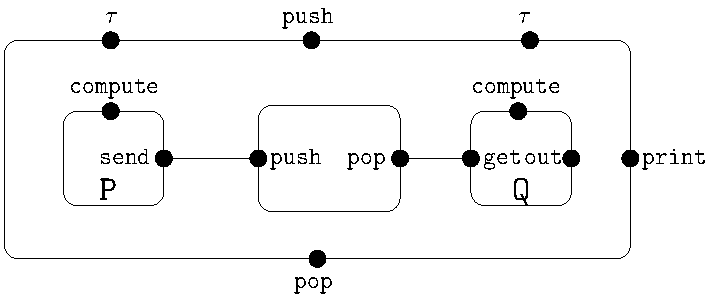
\includegraphics[width=.70\textwidth]{Figures/Architecture.pdf}
   \caption{Structure of the example. Each box corresponds to a process whose ports are the actions it can perform. The  actions observable by the environment are $\texttt{push}$, which indicates the enqueuing of an element, $\texttt{pop}$ which indicates the dequeuing, and $\texttt{print}$ which indicates the production of results. \label{Fig:Architect}} 
\end{figure}


The OA  modelling the behaviour of such a system  using an  unbounded circular/ring buffer is depicted in Fig. \ref{Fig:RefineOA}.  The automaton has a single state with  two holes: $\texttt{P}$ and  $\texttt{Q}$ that are the two interacting processes.  $\texttt{l}$ (as last)  indicates the next available position for  enqueuing an element  and  $\texttt{f}$ (as first) is the position that contains the next element to be dequeued. %\footnote{The  arrow  without any state of origin is a graphical convention to indicate that the pointers are initialized at the beginning}. 
The buffer reacts to a push from $\texttt{P}$ and enqueues it. Similarly, whenever   $\texttt{Q}$ pops an element, it dequeues it. Additionally, whenever $\texttt{Q}$ produces an item, it is exposed as an external observable  $\texttt{print}$ action. 
When any process do its internal computation, it is exposed externally as unobservable action $\tau$. 

The example uses several kinds of data. Variable $\texttt{m}$ holds a message (we can leave the message type abstract here). We additionally use arrays of messages with a syntax of the form $\texttt{M[l]}$ for array accesses; $\texttt{M}$ is an array of $\texttt{N}$ elements, from $0$ to $\texttt{N}-1$. Finally we use addition and modulo operation ($\%$) on integers.

\begin{figure}[!tb]
 \centering
   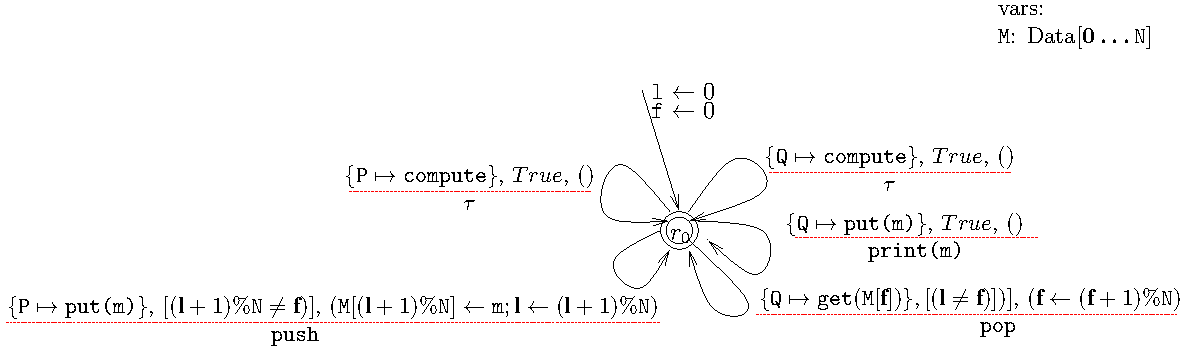
\includegraphics[width=.99\textwidth]{Figures/FIFORing.pdf}
   \caption{OA for the \texttt{prod-cons} system using FIFO circular buffer.
    \label{Fig:RefineOA}} 
\end{figure}
\qed
\end{example}





\paragraph{Open automata composition.}

OA are partially specified automata, the partiality arises  from the holes.
A hole can be seen as a port in which we can plug an OA.
The plugging operation is called composition.
The composition of OA was already implicitly defined by the means of composition on pNets in previous work \cite{henrio:01299562}. We provide here a (new) direct definition of composition for OA.




\begin{definition}[Composition of OA] \label{Def:CompOA}
% TODO: this definition is a bit strange, why is Ac in the hole of Ap but the hole is in Ac and the notation is reversed?
Let  \(A_c = \OAg[c]\) be an OA and $k$ one of its holes, \(k \in J_c\). Let \(A_p = \OAg[p]\) be another OA,  the composition $A_c\subst{A_p}{k}$ that fills the hole $k$ of the context OA \(A_c\) with the parameter OA \(A_p\) is defined as follows:
\[A_c\subst{A_p}{k} ::=  \OA{S_c \times S_p}{\mpar{s_{0c}, s_{0p}}}{V_c \uplus V_p}{\sigma_{0c} \uplus \sigma_{0p}}{J_p \uplus J_c \setminus \mbrc{k}}{T} \] \text{with }
\begin{align*}
T\!=& \mset{\OT{\mpar{s_c, s_p}}{\mpar{s'_c, s'_p}}{\alpha_c}{\beta_j^{j \in J'_p \uplus J'_c}\!}{g_c \wedge g_p \wedge \alpha_p = \beta_k}{\psi_c \uplus \psi_p}}{ \OT{s_c}{s'_c}{\alpha_c}{\beta_j^{j \in J'_c \uplus \mbrc{k} }\!}{g_c}{\psi_c} \in\! T_c, \OTx{p}{}{}{p} \in\! T_p} \\
	& \cup \mset{\OT{\mpar{s_c, s_p}}{\mpar{s'_c, s_p}}{\alpha_c}{\beta_j^{j \in J'_c}}{g_c}{\psi_c}}{\OTx{c}{}{}{c} \in T_c, k \notin J'_c, s_p \in S_p}
\end{align*}
\end{definition}

The first OA decides when the second can evolve by involving its hole in a transition: the action emitted when \(A_p\) makes a transition is synchronised with the action of the hole \(k\) in transitions of \(A_c\).
The condition $ \alpha_p = \beta_k$ ensures that the action emitted by the automaton $A_p$ filling the hole is the one expected in the hole $k$ of the open automaton $A_c$.




\begin{example} \label{Example:prodandcons} Fig. \ref{Fig:procandcons} shows a producer automaton  and a consumer  automaton that can be used  to fill the holes $\texttt{P}$ and $\texttt{Q}$ of \texttt{prod-cons} defined in Example~\ref{Example:fifo-system}.
 \begin{figure}[!t]
 \centering
   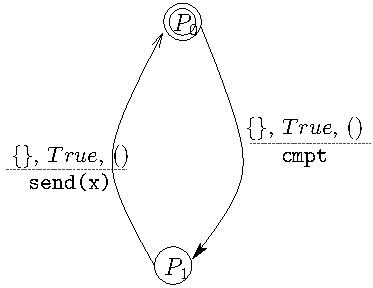
\includegraphics[width=.35\textwidth]{Figures/P-proc.pdf}\hfill 
   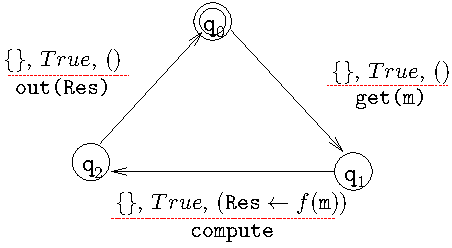
\includegraphics[width=.45\textwidth]{Figures/Q-proc.pdf}
   \caption{(Left) A \texttt{producer}.  It produces one item at a time and pushes it.  (Right)  A \texttt{consumer}. It pops an item, does some work and pushes the result. \label{Fig:procandcons}}
\end{figure}



The OA on Fig. \ref{Fig:ComposeOA} is the composition of the system in Fig.~\ref{Fig:RefineOA} and the producer in Fig. \ref{Fig:procandcons} (left). The composition consists of two states (the product of the states of both automata). The transitions from one state to another come from  the synchronisation  of the transitions of the encompassing automaton with those of the producer filling the hole $\texttt{P}$, this is why there is no more action from hole $\texttt{P}$ in the composed automaton. Only elements related to the hole $\texttt{P}$ are changed and in particular, transitions involving \texttt{Q} remain unchanged. \qed


\begin{figure}[!t]
 \centering
   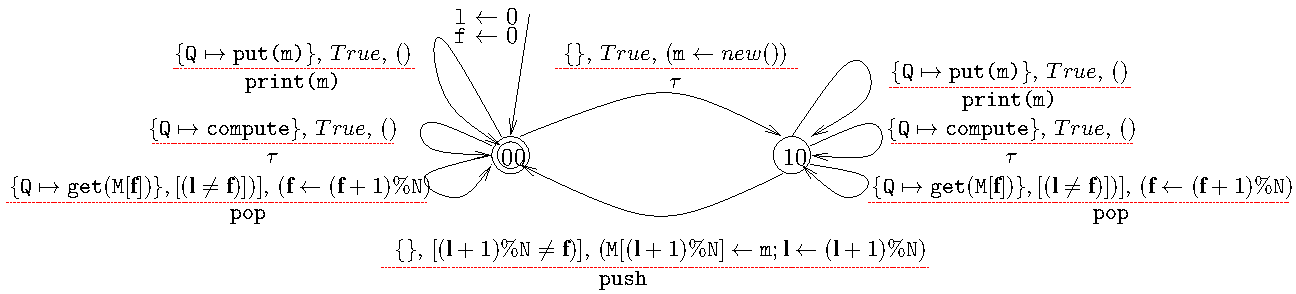
\includegraphics[width=.99\textwidth]{Figures/compos-FIFO-Pro.pdf}
   \caption{OA for filling the hole $\texttt{P}$ in \texttt{prod-cons}: \texttt{prod-cons}[\texttt{P}/\texttt{producer}]. 
   \label{Fig:ComposeOA}} 
\end{figure}
\end{example}



\subsection{Relations between Open Automata}
Establishing semantic equivalences and simulation relations between different OA requires  to compare their states. For this purpose, we suppose that the variables of the two OA are disjoint (a renaming of variables may have to be applied before comparing OA states).
\begin{definition}[Relation on open automata configurations] Suppose $V_1$ and $V_2$ are disjoint.
A relation on configurations of two OA \(\OAg[1]\) and \(\OAg[2]\) is a function \( \mathcal{R}: S_1 \times S_2 \to \rformulas[V_1 \uplus V_2]\).
\end{definition}
%\TODO{C'est etrange, la formulation "the variables they refer to", comme il n'y a plus de variables d'etat... +1}
The idea is that two states are related depending on the satisfiability of the expression relying their variables, i.e., if the variables of the OA verify a certain formula. 
In other words, to each pair of states is attached a boolean formula that may refer to the  variables of each of the two OA, stating whether the two states are related or not.
Additionally, we say that the relation $ \mathcal{R}$ \emph{relates the initial states} of the automata if: \(\sigma_{01} \uplus \sigma_{02} \models  \mathcal{R}\mpar{s_{01}, s_{02}}\).
We illustrate such a relation over automata with bisimulation relation below.

%\TODO{I do not think we reason on configurations for the moment, if we want to, we should introduce this:}
%Two configurations \(\mpar{s_1, \sigma_1} \in S_1 \times\mpar{V_1 \to \values}, \mpar{s_2, \sigma_2} \in S_2 \times \mpar{V_2 \to \values}\) are related iff \(\sigma_1 \uplus \sigma_2 \models R\mpar{s_1, s_2}\).

\subsection{A Bisimulation for Open Automata}

Bisimulation between OA was defined in~\cite{AMHEEMA:2023}.  We show below the principles of this bisimulation. We first recall the usual definition of bisimulation.
Bisimulation can  be defined as follows for standard transition systems: 

\begin{definition}[Classical Bisimulation]
  A bisimulation is a relation $\mathcal{R}$ such that if $s~\mathcal{R}~t$ then:\\
  \begin{minipage}[c]{.6\textwidth}
    \[
      \forall l~s',~ {s}\xrightarrow{l}{s'}
      \implies
      \exists t'.~ s' ~\mathcal{R}~ t'
      \land {t}\xrightarrow{l}{t'}
    \]
\begin{center}    \vspace{-1.5ex}
      and conversely
    \end{center}
    \vspace{-1ex}
    \[
      \forall l~t',~ {t}\xrightarrow{l}{t'}
      \implies
      \exists s'.~ s' ~\mathcal{R}~ t'
      \land {s}\xrightarrow{l}{s'}
    \]
    \vspace{.5ex}
  \end{minipage}
  i.e. \qquad
  \begin{minipage}[c]{.35\textwidth}
    \begin{tikzpicture}
      \node (s) at (-1,1) {$s$};
      \node (R) at (0,1) {$~\mathcal{R}$};
      \node (t) at (1,1) {$t$};
      \node (sp) at (-1,0) {$s^\prime$}
      edge [<-] node[auto] {$l$} (s);
      \node (Rp) at (0,0) {$\mathcal{R}$};
      \node (tp) at (1,0) {$t^\prime$}
      edge [<-] node[auto,swap] {$l$} (t);
    \end{tikzpicture}
  \end{minipage}
$s$ and $t$ are bisimilar, written $s\sim t$ iff there is a bisimulation relation $\mathcal{R}$ such that  $s ~\mathcal{R}~ t$.
If only the first one of the two implications above is verified, we say that $s$ simulates $t$ and denote it $s\leq t$.
\end{definition}

A  bisimulation relation  relates pair of states and ensures that any behaviour of one automaton can be performed by the other one while staying in relation. We informally explain here the symbolic nature of the bisimulation for OA and the related complexity of its definition.
The notion of symbolic bisimulation, as it was introduced in \cite{HENNESSY:1995}, is aimed at computing bisimulation of value-passing systems, i.e. systems made of processes exchanging data with their environment and between processes, where data are values from a possibly infinite domain.
 The presence of holes in fact raises no strong difficulty but the variables must be handled carefully.
Consider the two following simple OA:

\noindent~\begin{tikzpicture}
  \node[state,inner sep=5pt,minimum size=10pt] (1) {$s$};
  \node[state,inner sep=5pt,minimum size=10pt, below right of=1,right=90pt] (2) {$t$};
  \node[state,inner sep=5pt,minimum size=10pt, above right of=1,right=90pt] (3) {$t'$};

  \draw (1) edge[pos=.4] node[below=6pt]{\OTd{\alpha(x)}{h\mapsto\beta(x)}[x<0]{y\leftarrow -x}}  (2);
  \draw (1) edge[pos=.4] node[above]{\OTd{\alpha(x)}{h\mapsto\beta(x)}[x\geq 0]{y\leftarrow x}} (3);
\end{tikzpicture}
\hfill
\begin{tikzpicture}
  \node[state,inner sep=5pt,minimum size=10pt] (1) {$s_2$};
  \node[state,inner sep=5pt,minimum size=10pt,  right of=1,right=90pt] (2) {$t_2$};
\draw (1) edge[align=center] node[below]{\OTd{\alpha(x)}{h\mapsto\beta(x)}{z\leftarrow x}}  (2);
%  \draw (1) edge[align=center] node[above]{\OTd{\alpha(x)}{h\mapsto\beta(x)}{x\geq 0}{y\leftarrow x}} (3);
\end{tikzpicture}~

We should be able to consider these two OA as bisimilar. Both can input any $\beta(x)$ input on their hole and stores the value of $x$, emitting $\alpha(x)$ along the transition.
The difference is the way $x$ is stored. We can then define a configuration relation $\mathcal{R}$ such that $\mathcal{R}(s,s_2)$ is true and $\mathcal{R}(t,t_2)$ holds when $z\geq 0$ and $y=z$, while $\mathcal{R}(t',t_2)$ holds when $z< 0$ and $y=-z$. This illustrates relation on configurations, but also shows that bisimulation on OA is more complex than in the classical case. Indeed, we need two transitions on the left OA to simulate a single one on the right OA. We should check that these two transitions cover all the cases accepted by the right hand side OA, and of course that destination states are in relation. Formally, FH-bisimulation is defined as follows \cite{AMHEEMA:2023}:


 \begin{definition}[Strong FH-bisimulation]\label{def-FH-bisim} ~\\
\noindent
	Suppose  $\OAg[1]$ and $\OAg[2]$
%   $A_1 = \mylangle J,\mathcal{S}_1, s_0,V_1,
%   \mathcal{T}_1 \myrangle$ and $A_2 = \mylangle J,\mathcal{S}_2,t_0,V_2, \mathcal{T}_2 \myrangle$
   are OA with identical holes of the same sort, with disjoint sets of variables ($V_1\cap V_2=\emptyset$).  

 Then 
$\mathcal{R}$, a relation on configurations of OA, is an FH-bisimulation if and only if for any  states
$s\in{S}_1$ and $t\in{S}_2$, we 
have
the following:

 \begin{itemize}
 \item   
For any open transition $OT$ in ${T}_1$:
$
     \OTbase{s \OTarrow{\alpha} s'}
         {
           \beta_j^{j\in J'}}{g_{OT}}{\psi_{OT}}
$
 there exists an indexed set of  open transitions $OT_x^{x\in X} \subseteq {T}_2$:
$
%    \left( fresh \ \set{\alpha_i}, \set{b_j}, v_x.\ \
    \OTbase{t \OTarrow{\alpha_x} t_x}
         {
           \beta_{j x}^{j\in J_{x}}}{ g_{OT_x}}{\psi_{OT_x}}   
%         \right)
$
%\end{minipage}
%\hspace{2mm}
%\begin{minipage}{0.35\linewidth}
%\vspace{-2em}
%{	\includegraphics[width=1.02\linewidth]{XFIG/Bisim}}
%\end{minipage}
 such that  $\forall x.\, J'=J_{x}$ and there exists \hl{ $Pred_{s',t_x}$ such that} $\mathcal{R}(s',t_x)  
 $ holds \RAB{On n'a pas  de Pred dans la def}
 and  
\begin{multline*}
 \mathcal{R}(s,t) \land g_{OT}\implies\\
 \displaystyle{\bigvee_{x\in X}
   \left( \forall j. \beta_j=\beta_{jx}  \land g_{OT_x}
     \land \alpha\!=\!\alpha_x \land  
     \mathcal{R}\left(s',t_x\right)\psubst{\psi_{OT}\!\uplus\!\psi_{OT_x}}\right)}
\end{multline*}
     %     \symb{Subst}(\Pred_{target_x}, \Post_{OT} o \Post_{OT_x})
     %     \right)$.
%\bigskip
%
% $\Pred_{s,t} \land \Pred_{OT}\implies\bigvee_{x\in X} \Pred_x$
%and\\
%%\hspace{1cm}
% $ \forall{x\in X}. \Pred_x \land \Pred_{s,t} \land \Pred_{OT} \Rightarrow
%   \left( \forall j. \beta_j=\beta_{jx}  \land \Pred_{OT_x}
%     \land \alpha\!=\!\alpha_x \land  
%     \Pred_{s',t_x}\subst{\Post_{OT}\uplus\Post_{OT_x}}\right)$
%     %     \symb{Subst}(\Pred_{target_x}, \Post_{OT} o \Post_{OT_x})
%     %     \right)$.



%     \TODO{Eric: j'ai ajoute $\exists$ sur les predicats $\Pred_{s',t_x}$, qui n'etaient pas definis...}
     
 \item  and symmetrically any open transition from $t$ in ${T}_2$ can be 
      covered by a set of transitions from $s$ in ${T}_1$.
 \end{itemize}

Two automata are bisimilar if there exists a strong FH-bisimulation $ \mathcal{R}$ that relates their initial states.

% \TODO{Eric: il reste des petits bugs genre $s^{2'}_x$ plutot que
%   $s^{2}_x$}
 
%Where $\symb{Subst}(\Pred,\Post)$ is the parallel substitution of all
%assigned variables.

% \TODO{do we want formulas for this?}
 \end{definition}
Note that this definition matches an open transition $t_1$ to a family of covering open transitions $t_{2x}^{x\in X}$.
Intuitively, this means that for every pair of related
states $(s_1,s_2)$  of the two automata, and for every  transition of the first automaton from $s_1$, there is a set of matching transitions  of the second automaton  from $s_2$ such that the produced action match, the actions of the same holes and the successors are related after variable update.
Technically, the following sections do not rely on the definition of strong bisimulation on OA, but they follow the same principles and in particular the same way to faithfully simulate an open transition by a set of other open transitions.

%\begin{comment}
\subsection{Reachability}
We finally define a new predicate abstracting state reachability for OA, it  allows us to reason on reachable states in an automaton. It can  be seen as an abstraction of the reachable states under the form of a predicate that must stay verified along the execution of the OA.
\begin{definition}[Reachability] \label{Def:Reach}
For any OA \(A = \OAg\), a reachability predicate \(\reach{A}: S \to \rformulas[V]\) is any predicate on states that is valid on initial state, and preserved across transitions:
\[\sigma_0 \models \reach{A}\mpar{s_0}\quad\land\quad\forall t = \OTg \in T, \fvars{t} \models \left(\reach{A}\mpar{s} \wedge g \implies \reach{A}\mpar{s'}\psubst{\psi}\right)\]
\end{definition}

Reachability takes into account all paths, and can over-approximate the reachable configurations. 
From an automation point of view, finding the most precise reachability predicate for a given automaton is not decidable because of the symbolic nature of OA, but only an over-approximation is necessary.

%\end{comment}

\section{Simulation  for Automata with the Same Holes}\label{sec:refinement}

Similarly to FH-bisimulation~\cite{AMHEEMA:2023} we are interested  in finding simulation relations between configurations of two OA that contain variables and holes. When dealing with open systems it is common to define simulation in terms of a simulation relation.
We rely on a classical notion of simulation and perform the same extension as in~\cite{AMHEEMA:2023}, i.e. we start from a simulation relation and add holes and symbolic. The idea is to consider two configurations related by a relation; if one state can do a transition, then the other can also make this transition. 
Like for bisimulation, a simulation relation characterises when two states are related, and this  characterisation is expressed as a predicate on the variables of the two automata.
Simulation defines conditions on a relation $\mathcal{R}$ such that $\mathcal{R}\mpar{s_1, s_2}$ is a predicate (possibly involving variables of the automata) that is true when the state $s_1$ of $A_1$ simulates the state $s_2$ of $A_2$.


%\TODO{check deadlock reduction/reducing in the literature}

%
%\begin{definition}[Deadlock reduction]\label{def:dpwd}\\
%Let \(\OAg[1]\) and \(\OAg[2]\) be two OAs.
%A relation on OA configurations \(R: S_1 \times S_2 \to \rformulas[V_1 \uplus V_2]\) is deadlock reducing if  it satisfies the following\footnote{Note that variables of $T_1$ are existentially quantified in the proposition.}:
%\begin{multline*}
% \forall \mpar{s_1, s_2} \in S_1 \times S_2,
% \\ V_1 \uplus V_2 \uplus \biguplus_\subbox{t_2 \in \fOT{s_2}} \fvars{t_2} \models \left(R\mpar{s_1, s_2} \wedge \bigvee_\subbox{t_2 \in \fOT{s_2}} \fguard{t_2} \implies \bigvee_\subbox{t_1 \in \fOT{s_1}} \fguard{t_1} \right)
%\end{multline*}
%\end{definition}

%Because of the symbolic nature of OAs and their structure, in this definition,  the fact that a guard is true is sufficient to reason on the possible paths. This slightly simplifies the definition and makes the characterisation of transition that can be triggered very symbolic. An equivalent but more classical definition of deadlock reduction could be expressed as well. It states that if there is a transition that can be triggered in the first automaton, then there is a transition from the related state in the second automaton that can be triggered. This second definition is more verbose, in particular because of the multiple quantifiers over transitions and automaton state. The alternative definition is equivalent to this one when reasoning on a refinement relation (but not in general).

%Unfortunately, this property is not compositional: the composition operator can itself introduce a deadlock. In other words, when filling the hole of two related automata with a third one, even if there is a deadlock reduction between the two original automata, there might not be a deadlock reduction in the composed ones. The same problem may arise when two related automata are composed in the same hole of a third one. 
\begin{comment}

\TODO{add a notion of composable at hole i:
An OA is composable at hole k if it is partially deterministic relatively to actions of hole k
}
USEFUL for context only

\begin{multline*}
\forall s_1\in S,\, \forall \OTx{1}{a}{1}{1}, \OTx{1}{b}{2}{2} \in \fOT{s_1}.\\
\neg\left(\alpha_{1 a} = \alpha_{1 b}\land g_{1 a}\land g_{1 b} \land\beta_{1 k} \neq \beta_{2 k}\right)
\end{multline*}

A composable automaton cannot transform external non-determinism of the sub-automaton into internal non-determinism.

\end{comment}

%This creates a conflict between deadlock reduction and the properties involving composition. One possible solution to avoid this conflict is to only consider a composition that do not introduce deadlocks, we will define such a composition below.
%But before defining non-blocking composition, we first introduce a notion of state reachability for open automata. 

%
%\begin{definition}[Non-blocking composition]\label{Def:Non-blockcomp}
%Let \(A_i = \OAg[i]\) with \( 0 \leq i \leq n\) be a family of open automata.
%Let \(A = A_0\mdbrk{j_i \mapsto A_i \middle| 1 \leq i \leq n}\) and $A= \OAg$.
%
%The composition \(A_0\mdbrk{j_i \mapsto A_i \middle| 1 \leq i \leq n}\) is non-blocking if   \(A \) has a reachability predicate such that, for each reachable configuration, if there is a possible transition in \(A_0\) then there is a possible transition in \(A\):
%\[ \forall s = \mpar{s_0, s_1,..,s_n} \in S, V \uplus \biguplus_\subbox{t_0 \in \fOT{s_0}} \fvars{t_0} \models \left(\reach{A}\mpar{s} \wedge \bigvee_\subbox{t_0 \in \fOT{s_0}} \fguard{t_0} \implies \bigvee_\subbox{t \in \fOT{s}} \fguard{t} \right)\]
%\end{definition}
%Again we use guards to ensure that the transition can occur. It is not sufficient to ensure the existence of equivalent transitions in general, but it will be sufficient in the context of refinement.


%The idea is that 


%\subsection{Deadlock Reduction, Reachability, and Composition}

However here we want to build a simulation relation that  also guarantees that no deadlock is introduced when refining the automaton. This property is quite frequent in simulation relation, and referred to as \emph{lack of new deadlocks}~\cite{Kouchnarenko:2007} or \emph{complete simulation}~\cite{sangiorgi:bisim-coind12}.
The notion of deadlock should however be specialised to our OA. 
Indeed, it is not very useful to check the  existence of a transition, instead it makes more sense to use the guards to check if a transition can be taken.
 We thus define a deadlock reduction criterion based on how the outgoing transitions are guarded.
As such, a simulation does not introduce deadlocks if in the conditions where no transition is possible in the refined automaton, no transition were already possible in the more general one. More formally, for any pair of states $s_1$ and $s_2$  we introduce a criterion of the form: 
\begin{multline*}
\forall \mpar{s_1, s_2} \in S_1 \times S_2, \\
	V_1 \uplus V_2 \models \biggl( \mathcal{R}\mpar{s_1, s_2} \wedge \lnot \Bigl( \bigvee_\subbox{t_1 \in \fOT{s_1}} \fguard{t_1} \Bigr) \implies \lnot \Bigl( \bigvee_\subbox{t_2 \in \fOT{s_2}} \fguard{t_2} \Bigr) \biggr)
\end{multline*}


Which can be rewritten as:
\[
\forall \mpar{s_1, s_2} \!\in\! S_1 \!\times\! S_2, V_1 \uplus V_2
	\models\! \biggl(\! \mathcal{R}\mpar{s_1, s_2} \!\implies\! \Bigl(\!\! \bigvee_\subbox{t_1 \in \fOT{s_1}}\! \fguard{t_1} \Bigr) \lor \lnot \Bigl(\!\!  \bigvee_\subbox{t_2 \in \fOT{s_2}}\! \fguard{t_2} \Bigr) \!\biggr)
\]

Both statements being equivalent, as each of them may reveal more intuitive than the other in different situations, we  use them interchangeably.
%Let us first explain the reasons why simulation can introduce allow undesired behaviours to emerge and how we want to limit them. 
%The automaton that simulates a specification features any behaviour that contains the behaviour of the specification, or more precisely, for each state that simulates a state of the specification, the simulating automaton must at least feature the behaviour of the specification.
% In this definition, nothing prevents the implementation from 
%
%adding non-determinism and non-deterministically reaching a state that is unrelated to the specification, this state could even be a deadlock even though we only followed transitions that exist in the specification.
%To avoid the appearance of such deadlocks, we will state that, when both the implementation and the specification do the same transition, they stay related.
%This ensures a form of continuity in the comparison in the sense that the refined system is constrained to follow the behaviour of the simulated system along a given scenario. 
%In terms of traces this amounts to some form of deadlock reduction: for each trace followed by the simulated system if the refined system followed the beginning of the trace, it must be able to keep following the trace. 
%Of course, the classical trace view is a simplified view compared to the guards, states and actions from  the holes that exist in OA, but it gives the right intuition.
%
%Next definition states that if $T_2$ is not in a deadlock position then $T_1$ can do a transition but not necessarily with the same input values. This is very weak but sufficient when composed with the def  of simulation.
%\begin{definition}[Preservation along identical transitions]\label{def:preservation} \\
%Let \(\OAg[1]\) and \(\OAg[2]\) be two OAs.
%A relation \(R: S_1 \times S_2 \to \rformulas[V_1 \uplus V_2]\) between  \(\OAg[1]\) and \(\OAg[2]\)
%  is preserved along identical transitions if  it satisfies the following:
%\begin{multline*}
%\forall \mpar{s_1, s_2} \in S_1 \times S_2, \bigsymb{\forall} \mpar{t_1, t_2} = \mpar{\OTx{1}{}{1}{1}, \OTx{2}{}{2}{2}} \in \fOT{s_1} \times \fOT{s_2} \\  V_1 \uplus V_2 \uplus \fvars{t_1} \uplus \fvars{t_2} \models \hspace{6cm}\\  R\mpar{s_1, s_2} \wedge 	g_1 \wedge g_2 \wedge \alpha_1 = \alpha_2 \wedge \bigwedge_\subbox{j \in J'_1 \cap J'_2} \beta_{1j} = \beta_{2j} \implies  R\mpar{s'_1, s'_2}\psubst{\psi_1 \uplus \psi_2}\\
%\end{multline*}
%\end{definition}
%We thus define the following property that can be understood as follows. Take a specification automaton and its implementation. Consider two related states for the refinement relation. Suppose an identical transition exist in both automata (with same guards and same label), then either the reached states $s_1'$ and $s_2'$ are related by refinement, or there exists another transition of the specification that is also identical and leads to a state $s_1''$ that is related to $s_2'$ in the refinement relation.
%Finally, we should take into account that 1) instead of equality, we should check if there is a state such that both transitions are feasible (the conjunction of guards is satisfiable), and that  2) instead of finding another transition of the specification we might find a family of transitions that cover all the cases of the transition of the implementation. 
We can now state the definition of simulation between OA that have the same set of holes. 

\begin{definition}[Hole-equal simulation]\label{def:HoleEqualSim}
Consider two OA with identical set of holes:
\(A_1 = \OA{S_1}{s_{01}}{V_1}{\sigma_{01}}{J}{T_1}\) and \(A_2 = \OA{S_2}{s_{02}}{V_2}{\sigma_{02}}{J}{T_2}\), the relation on configurations \(\mathcal{R}: S_1 \times S_2 \to \rformulas[V_1 \uplus V_2]\) is a hole-\(\symb{equal}\) simulation from $A_1$ to $A_2$ if the following conditions hold : 
\item[(1)] \(\sigma_{01} \uplus \sigma_{02} \models \mathcal{R}\mpar{s_{01}, s_{02}}\)
\item[(2)] \(\forall \mpar{s_1, s_2} \in S_1 \times S_2,\)\vspace{-8pt}
\noindent\begin{multline*}
 \bigsymb{\forall} {t_1} = \OTx{1}{}{1}{1} \in \fOT{s_1} .\,~~
\bigsymb{\bigexists} 
\mpar{t_{2x} \!=\! \OTx{2}{x}{2x}{2x}}^{x \in X}\in \fOT{s_2}.\,~~\\[2pt]
\mpar{\forall x \in X, J'_{2x} = J'_1 } \nwedge\hfill\\[1pt]
%\everymath{\displaystyle}\begin{array}{l}
V_1 \uplus V_2 \uplus  \fvars{t_1} \models 
 \mathcal{R}\mpar{s_1, s_2} \wedge g_1 \implies
 \operatorname*{\bigsymb{\bigvee}}_{x \in X}
{\everymath{\displaystyle}
\mpar{\begin{array}{l}
			\alpha_{2x} = \alpha_{1} \wedge \bigwedge_\subbox{j \in J'_1} \beta_{2xj} = \beta_{1j} \nwedge\\[12pt]
			 g_{2x} \wedge\mathcal{R}\mpar{ s'_{1},s'_{2x}}\psubst{\psi_{2x} \uplus \psi_{1}}
		\end{array}} }
%\end{array} 
\end{multline*}
\item [(3)] Deadlock reduction:
\[
\forall \mpar{s_1, s_2} \!\in\! S_1 \!\times\! S_2, V_1 \uplus V_2
	\models\! \biggl(\! \mathcal{R}\mpar{s_1, s_2} \!\implies\! \Bigl(\!\! \bigvee_\subbox{t_1 \in \fOT{s_1}}\! \fguard{t_1} \Bigr) \lor \lnot \Bigl(\!\! \bigvee_\subbox{t_2 \in \fOT{s_2}}\! \fguard{t_2} \Bigr) \!\biggr)
\]
If there is a hole-equal simulation from $A_1$ to $A_2$, then we say that  $A_2$ simulates $A_1$; we  denote it $A_2\leq A_1$.
\end{definition}



 %Note also the second part of the conjunction of condition (2) expresses the deadlock reduction between automata (as introduced in Definition \ref{def:dpwd}).   
The first and second conditions coincide with the natural way to prove inductively that an automaton simulates another by starting with the initial state. The third condition ensures that  simulation  prevents the introduction of deadlocks.
\LUDO{Similarly to bisimulation, the second condition states that, for any transition of the simulating automaton $A_1$, it corresponds to a transition of the automaton $A_2$ that does the same thing and ends up in a similar state. However a family is needed in $A_2$ because of the symbolic nature of transitions, and because depending on the values of the variables, $t_1$ may correspond to different transitions in $A_2$.}
Our definition captures a simple simulation for OA with the same holes that is more expressive than a strict simulation since it matches a transition with a family of transitions. 
For example, with such a relation we are able to check the simulation between two OA that differ by duplicated states, removed duplicated transitions,  reinforced  guards, different variables, etc.
We will show in Section~\ref{sec:prop} that this simulation relation has good properties in terms of transitivity, compositionality, and reflexivity.

%The principle of the third requirement is that the relation allows new behaviour to be added in terms of new traces, but doesn't allow new deadlocks to
%be added, i.e., for every ``path'' of the specification (abstract automaton) the implementation (refined automaton) must not add deadlocks.

%This definition leads to a notion of simulation as refinement similar to the one used in LOTOS \cite{Brinksma:87} and called ``extension refinement''.
%The extension consists in adding new functionalities by preserving existing ones.
%In the context of LOTOS, a functionality is roughly an acceptable trace.
%In this context, the authors define refusal of the trace and constraint refinement so that there is no more refused trace in the refined system than in the original one. Slightly more formally, consider an automaton with transitions $s_0 \xrightarrowdbl{t}$, consider $\mathcal{T}_A$ the set of traces of an automaton $A$; one can define the refusal of a trace $t$ as a set of actions such that all actions in the set can be refused after the automaton $A$ has performed the steps in the trace $t$, more precisely $X$ is a refusal of a trace if $\exists s. s_0  \xrightarrowdbl{t} s \wedge \forall a \in X. s \not{\xrightarrow{a}}$.

%Considering an OA with no  hole and no guard, i.e., in case the definitions of open automata coincide with those of automata, the fact that $R$ is preserved along identical traces ensures that the set  of refusal of valid traces is smaller in the refined automaton than in the specification.


\begin{example} \label{example:fifo-system-one}
To illustrate the simulation  of OA, we consider a variation on the \texttt{prod-cons} example. Namely,  we suppose that  the two processes  \texttt{P} and  \texttt{Q} communicate through a one-place  buffer. Fig. \ref{Fig:SpecOA} shows the OA modelling this simpler version of the system, that we refer to as \texttt{simprod-cons}. 
\begin{figure}[!b]
 \centering
   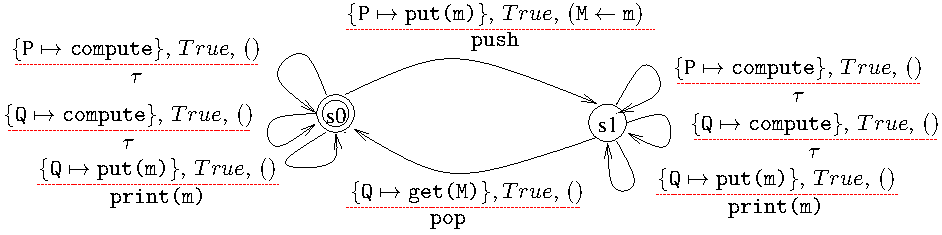
\includegraphics[width=.90\textwidth]{Figures/FIFOpen2.pdf}
   \caption{  The \texttt{simprod-cons} OA: the system using one-place  buffer.  \label{Fig:SpecOA}}
\end{figure}
We can easily check that this automaton simulates the one of Fig.~\ref{Fig:RefineOA}.
Indeed, one can see that  $\mathcal{R}=\{(r_0,s_0) \mapsto \texttt{l}=\texttt{f}, (r_0,s_1) \mapsto \texttt{f}=\texttt{l}+1\% \texttt{N} \}$ is  a  simulation 
relation. It follows that  \texttt{simprod-cons} $\leq$ \texttt{prod-cons}. \qed
\end{example}


%The refinement relation  also specifies that the refined process must follow the behaviour of the specification, not only at every compatible state but also along any scenario of the specification.


The simulation relation defined above is insufficient in the setting of composition which is the main advantage of the OA-based approach. Indeed, it should be possible to refine an automaton by filling its hole, providing a concrete view of a part of the application that was not specified originally. 
More generally, it should be possible to relate automata that do not have the same holes because composition is a crucial part of system specification.
%Thus, we believe composition should also be a form of refinement and call this feature \emph{refinement through composition}.
However, filling holes can result in a system with more or less holes than the original system because the plugged subsystem can contain itself many holes.
Next section  defines  a more powerful simulation relation able to reason on automata with different sets of holes.


%Technically,  it expresses how the concepts from the abstract and the refined systems are linked together.






\section{A Simulation Relation that Takes Holes into Account}\label{sec:holes}

This section  extends the preceding relation to automata where the set of holes is not the same. 
This is particularly useful  to state whether the automaton after composition is a simulation of the original automaton or not.
Indeed, when composing the set of  holes changes.
Being able to compare automata with only some of their holes in common seems useful in general.

\medskip
One major challenge in the extension of simulation to different sets of holes is to maintain a form of transitivity while being able to take into account the actions of some of the holes. A naive definition of simulation would ensure that only the holes that are identical in the two OA are taken into account in the simulation. Unfortunately, considering all the common holes does not ensure transitivity of the simulation for the following reason. If $A_1$ simulates $A_2$ and $A_2$ simulates $A_3$, and one hole $j$ appears in $A_3$ and in $A_1$ but not in $A_2$ then we have no guarantee on the way $A_1$ and $A_3$ take the actions of this  hole into account, thus  a simulation between and $A_1$ and $A_3$ would require conditions involving actions of the hole $j$ which cannot be ensured. The way we solve this issue is to remember in the simulation relation which holes have been compared. This makes the relation parameterised by a subset of the set of holes that belong to the two automata that we want to take into account.
This way, in the example above, we would have no guarantee on actions the hole $j$ by transitivity but can state a simulation relation with guarantees on the actions of the other holes.

In the following definition we add a parameter $H$ which is the set of holes tracked by the simulation relation and adapt the definition by ignoring actions of the holes that are not in $H$.
\LUDO{
Consequently, there is no guarantee related to the actions of the holes outside $H$.
We provide compositionality properties when plugging an automaton inside a hole in $H$ but cannot state anything when plugging an automaton outside $H$. The principle is that any property concerning holes that are not in $H$ should be proven specifically for the considered automaton or the considered composition of automata.
}

\begin{definition}[Hole-tracking simulation]\label{Def:OA-Refinement}
For two OA\\ \(A_1 = \OA{S_1}{s_{01}}{J_1}{V_1}{\sigma_{01}}{T_1}\) and \(A_2 = \OA{S_2}{s_{02}}{J_2}{V_2}{\sigma_{02}}{T_2}\), \(A_1\) is a simulation of \(A_2\) tracking holes \(H\), noted \(\wrel{A_1}{A_2}{H}\), with \(H \subseteq J_1 \cap J_2\), if there is a relation on configurations $\mathcal{R}: \mpar{S_1 \times S_2} \to \rformulas[V_1 \uplus V_2]$ such that\footnote{Note that the definition below is identical to the hole equal simulation except $\cap H$ is added in a few places.}:
\item[(1)] \(\sigma_{01} \uplus \sigma_{02} \models \mathcal{R}\mpar{s_{01}, s_{02}}\)
\item[(2)] \(\forall \mpar{s_1, s_2} \in S_1 \times S_2,\)
\begin{multline*}
	\everymath{\displaystyle}\begin{array}{l}
		\bigsymb{\forall} \OTx{1}{}{1}{1} \in \fOT{s_1}, \bigsymb{\exists} \mpar{\OTx{2}{x}{2x}{2x} \in \fOT{s_2}}^{x \in X}, \\[12pt]
		 \mpar{\forall x \in X, J'_{2x} \cap H = J'_1 \cap H} \nwedge\hfill\\[1pt]
		 V_1 \uplus V_2 \uplus \fvars{t_1} \models\\\hspace{5em} \mpar{\mathcal{R}\mpar{s_1, s_2} \wedge g_1 \implies \operatorname*{\bigsymb{\bigvee}}_{x \in X} \mpar{\begin{array}{l}
			\alpha_1 = \alpha_{2x} \wedge \bigwedge_\subbox{j \in J'_{1} \cap H} \beta_{1j} = \beta_{2xj}   \nwedge\\
			 g_{2x} \wedge \mathcal{R}\mpar{s'_1, s'_{2x}}\psubst{\psi_1 \uplus \psi_{2x}}
		\end{array}}} 
	\end{array} 
\end{multline*}
\item[(3)] Deadlock reduction:
\[
\forall \mpar{s_1, s_2} \!\in\! S_1 \!\times\! S_2, V_1 \uplus V_2
	\models\! \biggl(\! \mathcal{R}\mpar{s_1, s_2} \!\implies\! \Bigl(\!\! \bigvee_\subbox{t_1 \in \fOT{s_1}}\! \fguard{t_1} \Bigr) \lor \lnot \Bigl(\!\! \bigvee_\subbox{t_2 \in \fOT{s_2}}\! \fguard{t_2} \Bigr) \!\biggr)
\]
\end{definition}
Note that every action of the holes outside \(H\) is unconstrained according to the simulation relation.

%\begin{example} It is easy to see the  open automaton of Fig.~\ref{Fig:RefineOA} is a refinement the open automaton of Fig.~\ref{Fig:SpecOA} according to this definition.
%\end{example}

\begin{property}[Relating simulations]\label{lem-sim-sim}
Hole-equal simulation is a particular case of hole-tracking simulation when  $J_1=J_2=H$.
\end{property}
\LUDO{
In particular, if an OA has no holes, the two definitions are equivalent and result in a  ``symbolic simulation'', if additionally there is no variable in the OA, we obtain the classical simulation of process algebra theory.}


\begin{example} Consider the automata of Examples \ref{Example:fifo-system} and \ref{example:fifo-system-one}. As we saw above, \texttt{simprod-cons} $\leq$ \texttt{prod-cons}, therefore \texttt{prod-cons} $\leq_{\{\texttt{P,Q}\}}$ \texttt{simprod-cons}.
\end{example}
%\TODO{potential ex 4: check if the example with a hole filled is a simulation of the example with holes? }



%
%\TODO{
%A string $t \in \mathcal{A}^*$ is a trace of an automaton if there is some state $s$ such that $s_0 \xrightarrowdbl{t}  s$. We denote the set of traces of an automaton $A$ by $\mathcal{T}_A$. \\
%Notion of Extension refinement. May be we need to introduce the notion of  refusal of
%a trace $t \in \mathcal{T}_A$ is a set of actions such that all actions in the set can be refused after the automaton $A$
%has executed the trace $t$. \[X \in \bot_{A}(t) \Leftrightarrow \{\exists s. s_0  \xrightarrowdbl{t} s \wedge \forall a \in X. s \not{\xrightarrow{a}}    \}\] and replace deadlock reducing, under (3) by
%\[\forall t \in \mathcal{T}_{A_1} \cap  \mathcal{T}_{A_2},\, \bot_{A_2}(t) \subseteq  \bot_{A_1}(t)  \] } 
%
%\TODO{thm: backward compatibility + simulation is equivalent to extension refinement in case there is no hole and no guard, i.e. in case the definitions of automata coincide}

\begin{property}[Tracked holes] By construction, if an automaton is the simulation of another one, it is also a simulation by tracking less holes.
\[\wrel{A_1}{A_2}{H} \land H'\subseteq H \implies \wrel{A_1}{A_2}{H'}\]
\end{property}

Now that we have a simulation relation that takes both variable parameters and process parameters into account, we would like to ensure that it has  properties one would expect for a simulation relation.

\section{Properties of our Simulation Relations}\label{sec:prop}

Before reasoning on the properties of simulation, we need to introduce one additional notion that characterises when the composition of two automata does not introduce new blocked transitions.

\subsection{Non-blocking Composition}

%A notion that is often used in the context of refinement is the notion of deadlock reduction. This property considers that two states related by a given relation and states that if one state can do a transition, then the other can do a transition too. This notion is not much interesting in the general case as there is a priori no relation between the two transitions. However, when the relation that relates states is a simulation, this will relate the possible transitions and the deadlock reduction will become a valuable property.
\begin{comment}

Next definition states that if $T_2$ is not in a deadlock position then $T_1$ can do a transition but not necessarily with the same input values. This is very weak but sufficient when composed with the def  of simulation.

\TODO{remove this def}
\begin{definition}[Deadlock reduction]\label{def:dpwd}\\
Let \(\OAg[1]\) and \(\OAg[2]\) be two OAs.
A relation on OA configurations \(R: S_1 \times S_2 \to \rformulas[V_1 \uplus V_2]\) is deadlock reducing if  it satisfies the following\footnote{Note that variables of $T_1$ are existentially quantified in the proposition.}:
\begin{multline*}
 \forall \mpar{s_1, s_2} \in S_1 \times S_2,\\ V_1 \uplus V_2 \uplus \biguplus_\subbox{t_2 \in \fOT{s_2}} \fvars{t_2} \models \left(R\mpar{s_1, s_2} \wedge \bigvee_\subbox{t_2 \in \fOT{s_2}} \fguard{t_2} \implies \bigvee_\subbox{t_1 \in \fOT{s_1}} \fguard{t_1} \right)
\end{multline*}
\end{definition}

Because of the symbolic nature of OAs and their structure, in this definition,  the fact that a guard is true is sufficient to reason on the possible paths. This slightly simplifies the definition and makes the characterisation of transition that can be triggered very symbolic. An equivalent but more classical definition of deadlock reduction could be expressed as well. It states that if there is a transition that can be triggered in the first automaton, then there is a transition from the related state in the second automaton that can be triggered. This second definition is more verbose, in particular because of the multiple quantifiers over transitions and automaton state. The alternative definition is equivalent to this one when reasoning on a refinement relation (but not in general).
\end{comment}

Unfortunately, the deadlock reduction property in the definition of simulation is not compositional: the composition operator can itself introduce a deadlock. In other words, when filling the hole of two related automata with a third one, even if there is a deadlock reduction between the two original automata, there might not be a deadlock reduction in the composed ones. The same problem may arise when two related automata are composed in the same hole of a third one. 

This creates a conflict between deadlock reduction and the properties involving composition. 
%One possible solution to avoid this conflict is to only consider a composition that do not introduce deadlocks, we  define such a composition below.
%But before defining non-blocking composition, we first introduce a notion of state reachability for open automata. 
%\begin{definition}[Reachability] \label{Def:Reach}
%For any open automata \(A = \OAg\), a reachability predicate \(\reach{A}: S \to \rformulas[V]\) is any predicate on states that is valid on initial state, and preserved across transitions:
%\[\sigma_0 \models \reach{A}\mpar{s_0}\quad\land\quad\forall t = \OTg \in T, \fvars{t} \models \left(\reach{A}\mpar{s} \wedge g \implies \reach{A}\mpar{s'}\psubst{\psi}\right)\]
%\end{definition}
%Reachability takes into account all paths, and can over-approximate the reachable configurations. 
%From an automation point of view, finding the most precise reachability predicate for a given automata is not decidable because of the symbolic nature of open automata, but only an over-approximation is necessary. An automatic tool would only need to find an over approximation of reachability to reason on composition that is compatible with deadlock reduction. 
We call \emph{non-blocking composition} a composition that can  safely be used to compose OA that are involved in a deadlock reducing relation.

%\begin{definition}[Non-blocking composition] \label{Def:Non-block}
%Let \(A_i = \OAg[i]\) with \( 0 \leq i \leq n\) be a family of open automata.
%Let \(A = A_0\mdbrk{j_i \mapsto A_i \middle| 1 \leq i \leq n}\) and $A= \OAg$.
%
%The composition \(A_0\mdbrk{j_i \mapsto A_i \middle| 1 \leq i \leq n}\) is non-blocking if   \(A \) has a reachability predicate such that, for each reachable configuration, if there is a possible transition in \(A_0\) then there is a possible transition in \(A\):
%\begin{multline*}
% \forall s = \mpar{s_0, s_1,..,s_n} \in S, V \uplus \biguplus_\subbox{t_0 \in \fOT{s_0}} \fvars{t_0} \models \\ \left(\reach{A}\mpar{s} \wedge \bigvee_\subbox{t_0 \in \fOT{s_0}} \fguard{t_0} \implies \bigvee_\subbox{t \in \fOT{s}} \fguard{t} \right)
%\end{multline*}
%\end{definition}
\begin{definition}[Non-blocking composition] \label{Def:Non-block}
Consider two OA:\\ \(A_1 = \OAg[1]\) and \( A_2 = \OAg[2]\).
Let $A$ be the OA resulting from the composition \(A = A_1\subst{A_2}{k}= \OAg\). 
The composition \(A_1\subst{A_2}{k}\) is non-blocking if   \(A \) has a reachability predicate such that, for each reachable configuration, if there is a possible transition in \(A_1\) then there is a possible transition in \(A\):
%\begin{multline*}
\[ \forall s = \mpar{s_1, s_2} \in S, V \uplus \biguplus_\subbox{t \in \fOT{s_1}} \fvars{t} \models  \biggl(\reach{A}\mpar{s} \wedge \bigvee_\subbox{t \in \fOT{s_1}} \fguard{t} \implies \bigvee_\subbox{t \in \fOT{s}} \fguard{t} \biggr)
\]
%\end{multline*}
\end{definition}
Like in the definition of simulation (Definition~\ref{def:HoleEqualSim}) we use guards to ensure that the transition can occur. 
In general, one would not want to only consider non-blocking composition as it may reveal a bit restrictive, but it is the best necessary condition that we could  identify for compositionality of simulation. It will be used to prove composition theorems given below. 
In absence of non-blocking composition, simulation may also be checked specifically for a given composed automaton.
%It is not sufficient to ensure the existence of equivalent transitions in general, but it will be sufficient in the context of refinement.


\subsection{Properties}

We now  state the properties of our simulation, their formal proofs  can be found in  the extended version of this paper \cite{henrio:hal-04193421}. We express these properties  in terms of hole-tracking simulation because, thanks to Property~\ref{lem-sim-sim}   all the properties  of hole-tracking simulation are also valid  for hole-equal simulation.
The first crucial theorem of  simulation  is that it is  a  preorder on the set of OA. This latter enables stepwise refinement.


\begin{theorem}[Simulation is a preorder]\label{thm:preoder}
Hole-tracking simulation
   is reflexive  and  transitive:  it  is  a  preorder on the set of OA.
\end{theorem}

\begin{proofsketch}
% TODO: I don't understand this definition, why v = v on vars(s1), what about s2
% ANS: was copy paste from the report, polished now
 
The relation  \(\wrel{}{}{H}\) is reflexive,  \(\wrel{A}{A}{H}\). This is shown  by considering the relation $\mathcal{R}$ such that $\mathcal{R}\mpar{s_1, s_2} \triangleq s_1=s_2\land \displaystyle\bigwedge_\subbox{v \in vars(s_1)} {v=v}$   we can prove the conditions for Definition~\ref{Def:OA-Refinement}.
%
%\begin{theorem}[Transitivity]
%If $\wrel{A_1}{A_2}{H}$ and $\wrel{A_2}{A_3}{H'}$, then $\wrel{A_1}{A_3}{H\cap H'}$.
%\end{theorem}
In \cite{henrio:hal-04193421}, we give proof of transitivity. It is done classically by identifying the relation between $A_1$ and $A_3$ that is a simulation. What is less classical is the definition of this relation because it is a boolean formula. For each couple of states  $s_1$ and $s_3$ of $A_1$ and $A_3$ we build a  formula that defines the simulation. To do this, we take the disjunction of formulas relating $s_1$ and $s_3$, and passing by all states $s_2$ of $A_2$. More precisely, we define a relation of the following form:
  \[\mathcal{R}_{13}(s_1,s_3)=\bigvee_{s_2\in S_2}\left(\mathcal{R}_{12}(s_1,s_2) \land \mathcal{R}_{23}(s_2,s_3) \right) \]
We then prove that this relation  is a simulation, according to Definition~\ref{Def:OA-Refinement}.
\end{proofsketch}

The next  theorem states that if two automata are in simulation relation and the same automaton is placed in the same hole of the two automata, then the simulation is preserved. This is the first step toward proving that
 simulation is compositional in the sense that it is sufficient to prove simulation for the composed automata separately to obtain a simulation relation.
%The second part,  proving that placing in the same context two OA in simulation, we obtain two OA in simulation is left for future works.
%
%
%The composition of $A_1$ and $A_3$ is a refinement of the composition of $A_2$ and $A_3$ provided $A_1$ is a refinement of $A_2$ and the hole in which we are composing inside $A_1$ and $A_2$ is tracked by the refinement relation.



\begin{theorem}[Context refinement]\label{thm:ContextRefinement}
Let $A_1$, $A_2$ and $A_3$ be three OA with $\wrel{A_1}{A_2}{H}$. 
Let $J_3$ be the set of holes of $A_3$ and suppose that $k \in H$.
Suppose additionally that  \(A_1\subst{A_3}{k}\) is non-blocking.
We have: \[\wrel{A_1\subst{A_3}{k}}{A_2\subst{A_3}{k}}{J_3 \uplus H \setminus \mbrc{k}}\]
\end{theorem}



%
%
%
%
%\begin{theorem}[Congruence]\label{thm:Congruence}
%Let $A_1$, $A_2$ and $A_3$ be three open automata with $\wrel{A_2}{A_3}{H}$. 
%%Suppose that \(k \in H\) and that \(A_1\subst{A_2}{k}\) is non-blocking.
%We have: \[\wrel{A_1\subst{A_2}{k}}{A_1\subst{A_3}{k}}{J_1 \uplus H \setminus \mbrc{k}}\]
%\end{theorem}

%\TODO{i did not put the global composition theorem, de we state it?}


\begin{proofsketch}
The proof relies on a simulation relation that we consider is the one that makes $A_1$ and $A_2$ similar, complemented with identity of configurations for $A_3$.
Then, by construction, all transitions of the composed automaton $A_1\subst{A_3}{k}$ are specified by open transitions of $A_1$. For the transitions that do not involve hole $k$, the transition of $A_1\subst{A_3}{k}$ is the same and simulation between $A_1$ and $A_2$ allows us to conclude directly. If the hole $k$ is involved the considered relation  implies that valuations in $A_3$ are equal (i.e., the value for each variable are the same in both valuations), after a transition we should obtain ``equal'' valuations because post-conditions are deterministic. \RAB{The requirement $A_1\subst{A_3}{k}$ ensures  compatibility with deadlock reduction, i.e., it ensures that deadlocks in the refined model  are not introduced through composition.}
\end{proofsketch}

\begin{example}  Consider again the \texttt{prod-cons} and \texttt{simprod-cons}  automata given in the examples above.  Since  \texttt{prod-cons} $\leq_{\{\texttt{P,Q}\}}$ \texttt{simprod-cons},  then according to Theorem \ref{thm:ContextRefinement}, 
\texttt{prod-cons[producer/P]} $\leq_{\{\texttt{Q}\}}$  \texttt{simprod-cons[producer/P]}. 
The automaton of \texttt{prod-cons[producer/P]} is shown in Fig.~\ref{Fig:ComposeOA}. The automaton resulting  from the composition of  \texttt{simprod-cons} and \texttt{producer} is bigger and not shown here. \qed
\end{example}


\begin{theorem}[Congruence]\label{thm:CongurenceRefinement}
Let $A_1$, $A_2$ and $A_3$ be three OA with $\wrel{A_2}{A_3}{H}$. 
  Let $J_1$ be the set of holes of $A_1$ and suppose that \(k \in J_1\). Suppose additionally that the composition $A_1\subst{A_2}{k}$ is non-blocking.
We have: \[\wrel{A_1\subst{A_2}{k}}{A_1\subst{A_3}{k}}{J_1 \uplus H \setminus \mbrc{k}}\]
\end{theorem}

Consequently, as the simulation is transitive we can compose the previous theorems and  state the following: 
\begin{theorem}[Composability]\label{thm:Composability}
Let $A_1$, $A_2$, $A_3$ and $A_4$ be four OA with $\wrel{A_1}{A_2}{H}$ and $\wrel{A_3}{A_4}{H'}$.  Suppose that \(k \in H\). We have: \[\wrel{A_1\subst{A_3}{k}}{A_2\subst{A_4}{k}}{ H \uplus H'\setminus \mbrc{k}}\]
\end{theorem}

\begin{example}
As an example of the use of this theorem, if we design a refined version of the producer process of Example~\ref{Example:prodandcons} called $\texttt{Refproducer}$. According to  Theorem \ref{thm:Composability}, we have 
\texttt{prod-cons[producer/P]} $\leq_{\{\texttt{Q}\}}$  \texttt{simprod-cons[$\texttt{Refproducer}$/P]}. 
%as well as \texttt{prod-cons[P/producer]} $\leq_{\{\texttt{Q}\}}$  \texttt{Simprod-cons[P/$\texttt{producer}^{\flat}$]}.
\end{example}


%\begin{figure}[h]
% \centering
%   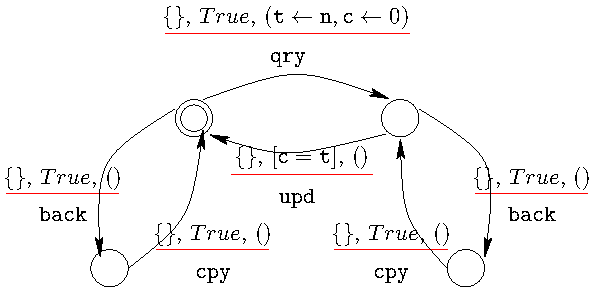
\includegraphics[width=.6\textwidth]{Figures/composeRefined.pdf}
%   \caption{Open automata resulting from the composition of the  refined  \texttt{database} and the \texttt{counter} \label{Fig:ComposeRefine}}
%\end{figure}



% TODO: why is there several ovoid stacked only on one side?
%\begin{center}
%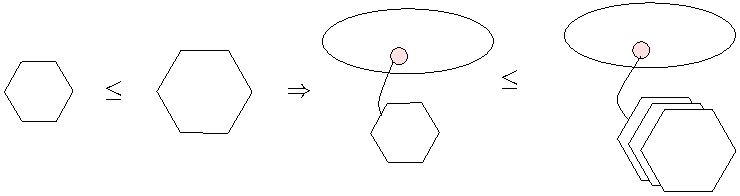
\includegraphics[scale=0.7]{Figures/Theorem1}
%\end{center}

%% TODO: non-blocking is not defines afaik
%% ANS: remove this from the submission because proof unfinished
%Open automata composition is a refinement where
%the tracked holes are the holes of the base automaton minus the composed hole.
%\begin{theorem}[Composition is a refinement]\label{thm:Composition}
%Let $A_1$ and  $A_2$  be three two automata with $J_1$ the set of holes of $A_1$.
%Suppose that \(k \in J_1\) and that \(A_1\subst{A_2}{k}\) is non-blocking. We have:
%\[ \wrel{A_1\subst{A_2}{k}}{A_1}{J_1\setminus \{k\}}\]
%\end{theorem}


%TODO: FOCUS on the two following items (look at quentin's article):
%
%
%- what is the property wrt deadlocks?
%
%
%- relation with fh bisimulation

Note that the substitution operation can be extended to a multiple substitution that fills several holes at the same time, and the theorems can be adapted accordingly.

%\TODO{parler de generalisation a la composition a n automates}

\section{Related Work}
\label{sec:sota}



The origins of refinement are in the  approach of programming that aims to provide solid foundations for building correct programs \cite{Dijkstra76}.  Many work  contributed to the  development of elaborated notions of refinement  in various area (e.g. \cite{BACK1990133,Abrialbooks96,soton250550,Bellegarde:2000}).
In the context of process algebra, refinement between processes can be defined in terms of simulations relation (e.g. (\cite{Jifeng:1089,Milner:1980}). However, the concept of simulations presented so far has focused on the refinement of systems that are inherently closed, i.e., systems which are bounded and without environment,

The simulation  ensures the preservation of   
safety properties as deadlock-freeness  and, more generally, 
all linear temporal logic properties \cite{Abrialbooks96,Kouchnarenko:2007}.
The difference between the existing refinement principles have been studied in \cite{10.5555/640428.640430}, for example the authors explain in what sense failure semantics is different from  (bi)simulation in the compared systems and properties ensured. In this paper we particularly focus on the compositionality of simulation-based refinement.
 
There are not a lot of works that study refinement for open systems. Defining refinement of open systems as trace inclusion  is  addressed  as a notion of subtyping in type theory 
(e.g. \cite{GayH:2005,BravettiZ:2021}). The definition of refinement is based on a connection  between session types and communicating automata theories -- a notion of session automata
based on Communicating Finite-State Machines, that are used for  modelling processes communicating through FIFO channels.    The refinement of open systems is also defined in terms of  alternating simulation \cite{Alur:1998,deAlfaro:2021}.
Alternating simulation  is originating from the game theory \cite{deAlfaro:2003}, it allows  the study of relation between individual components by viewing them as alternating transition systems. In particular,  a refinement of game-based automata expresses that the refined component can offer more services (input actions) and fewer service demands (output actions). However, the composition of such automata may
lead to illegal states, where one automaton issues an output that is not acceptable as input in the other one. The theory of alternating simulation provides an optimistic approach to compute compatibility between automata based on the fact that each automaton expects the other to provide  legal inputs, i.e., two components can be composed if there is an environment where they can work together. Our approach  has some commonalities with  the above mentioned simulation \cite{deAlfaro:2021}: both are process-oriented approaches even if they are not based on the same notion of simulation, and both include in the model  how to compose and interact with processes that are accepted as parameters.   Nevertheless, they differ in that our approach focuses on the compositional properties of the simulation, and {not on the fact that entities can be composed}.
% \LUDO{\st{TODO: what do we do better . in a different context?}}.

 
Previous works on OA focused on equivalence relations compatible with composition.
In  \cite{10.1145/3372884.3373161}, a computable bisimulation is introduced, while in \cite{AMHEEMA:2023}  a weak version of the bisimulation is introduced. 
In this paper we tackle the refinement relation in the form of simulation, as is the case for the corresponding relations on labelled transition systems \cite{Bellegarde:2000}. Unlike the standard simulation we deal with symbolic and open models. In \cite{Zhang2014}, the authors exploit transition systems to reason about the systems  that are partially specified by using variables, making  the state space potentially infinite.


%
%\LUDO{rewrite the following, relate non-blocking and the citation, is it the good one}
%\LUDO{add reference to Olga for non blocking but she does not ensure compositionality in a very general sense as we do}

{Some work target component-based refinement  with the concern  of preserving  deadlock freedom (e.g. \cite{DIHEGO2020110598,Kouchnarenko:2007}). These works are not concerned with the theory of open symbolic systems, and therefore do not focus on the same modularity as we do, in particular we provide preservation of refinement by composition.
}
%
%\TODO{A virer -- For example,  \cite{DIHEGO2020110598}  presented a refinement relation on process algebra based on. Indeed, failure semantics is based  on a notion of decorated traces.  Consequently, in this semantics,  refinement is defined in terms of inclusions between their decorated traces,  rather than by simulation.}


  
 





\section{Conclusion}\label{sec:ccl}
In this article we investigated the notion of refinement for a symbolic and open model: open automata. 
OA are convenient for compositional software verification. Indeed, OA  model parallel systems that are parameterised both by the use of variables and by the possibility to compose automata. The formalism supports compositional specification through the simulation paradigm.
In this paper, we introduce a refinement relation  between open automata. It relies on a simulation relation between the two automata;  it  specifies that the refined process must follow the behaviour of the simulated one. We finally showed that simulation is a preorder that is preserved by composition, both when filling a hole and when placing automata in comparable contexts.

%In the future, we want to investigate under which condition, the composition operation produces a refinement in the sense that filling a hole produces a refined process.




 \bibliographystyle{splncs04}
 \bibliography{biblio}






\end{document}
